\section*{Proposed Techniques}

\begin{frame}{Proposed technique: \CPDSearch{}}
    \begin{block}{Idea}
        Exploit the original CPD for the new perturbated map.
    \end{block}

    \begin{itemize}
        \item<2-> {\color<3->{gray}Use CPD as a concrete (suboptimal) solution};
        \item<3-> {\color<4->{gray}use CPD as an admissible heuristic};
        \item<4-> {\color<5->{gray}use CPD for a (early) search termination};
        \item<5-> {use CPD to obtain anytime solution (if weights $\not = \infty$)};
    \end{itemize}

    \only<3>{
        Given start, target $(s, t)$, since perturbations only increases edge costs, the cost of the shortest path computed by the CPD is a lowerbound of the actual shortest path in the perturbated graph;
    }%
    \only<2-3>{
        \begin{minipage}{0.5\textwidth}
            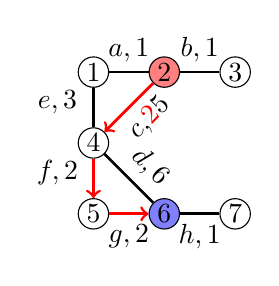
\begin{tikzpicture}
                \tikzset{Vertex/.style={%
                    shape=circle,%
                    draw=black,%
                    minimum size=10pt,%
                    radius=0.7cm,%
                    inner sep=1pt,%
                    node distance=0.9cm,%
                }}
            
                \node[Vertex] (1) {$1$};
                \node[Vertex, right of=1, fill=red!50] (2) {$2$};
                \node[Vertex, right of=2] (3) {$3$};
                \node[Vertex, below of=1] (4) {$4$};
                \node[Vertex, below of=4] (5) {$5$};
                \node[Vertex, right of=5, fill=blue!50] (6) {$6$};
                \node[Vertex, right of=6] (7) {$7$};
        
                \path (2) edge[-,line width=1pt] node[above]{\color{black}$a,1$} (1);
                \path (2) edge[-,line width=1pt] node[above]{\color{black}$b,1$} (3);
                \path (2) edge[->,line width=1pt, color=red] node[below,sloped,pos=0.4]{{\color{black} $c,$}{\color{red} \xcancel{2}}{\color{black}5}} (4);
                \path (4) edge[-,line width=1pt] node[above,sloped,pos=0.6]{\color{black}$d,6$} (6);
                \path (1) edge[-,line width=1pt] node[above,xshift=-13pt,yshift=-6pt]{\color{black}$e,3$} (4);
                \path (4) edge[->,line width=1pt, color=red] node[above,xshift=-13pt, yshift=-6pt]{\color{black}$f,2$} (5);
                \path (5) edge[->,line width=1pt, color=red] node[below]{\color{black}$g,2$} (6);
                \path (6) edge[-,line width=1pt] node[below]{\color{black}$h,1$} (7);
            \end{tikzpicture}
        \end{minipage}\hfill%
        \begin{minipage}{0.5\textwidth}
            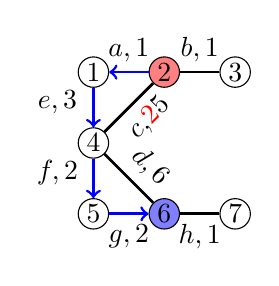
\begin{tikzpicture}
                \tikzset{Vertex/.style={%
                    shape=circle,%
                    draw=black,%
                    minimum size=10pt,%
                    radius=0.7cm,%
                    inner sep=1pt,%
                    node distance=0.9cm,%
                }}
            
                \node[Vertex] (1) {$1$};
                \node[Vertex, right of=1, fill=red!50] (2) {$2$};
                \node[Vertex, right of=2] (3) {$3$};
                \node[Vertex, below of=1] (4) {$4$};
                \node[Vertex, below of=4] (5) {$5$};
                \node[Vertex, right of=5, fill=blue!50] (6) {$6$};
                \node[Vertex, right of=6] (7) {$7$};
        
                \path (2) edge[->,line width=1pt, color=blue] node[above]{\color{black}$a,1$} (1);
                \path (2) edge[-,line width=1pt] node[above]{\color{black}$b,1$} (3);
                \path (2) edge[-,line width=1pt] node[below,sloped,pos=0.4]{{\color{black} $c,$}{\color{red} \xcancel{2}}{\color{black}5}} (4);
                \path (4) edge[-,line width=1pt] node[above,sloped,pos=0.6]{\color{black}$d,6$} (6);
                \path (1) edge[->,line width=1pt, color=blue] node[above,xshift=-13pt,yshift=-6pt]{\color{black}$e,3$} (4);
                \path (4) edge[->,line width=1pt, color=blue] node[above,xshift=-13pt, yshift=-6pt]{\color{black}$f,2$} (5);
                \path (5) edge[->,line width=1pt, color=blue] node[below]{\color{black}$g,2$} (6);
                \path (6) edge[-,line width=1pt] node[below]{\color{black}$h,1$} (7);
            \end{tikzpicture}
        \end{minipage}
    }%
    \only<4>{
        \begin{minipage}{0.5\textwidth}
            \begin{flushleft}
                path in original map: 6 \\
                path in perturbated map: 9
            \end{flushleft}
            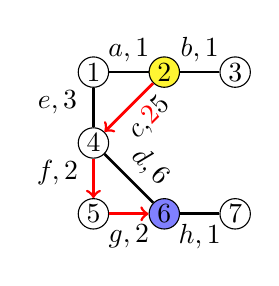
\begin{tikzpicture}
                \tikzset{Vertex/.style={%
                    shape=circle,%
                    draw=black,%
                    minimum size=10pt,%
                    radius=0.7cm,%
                    inner sep=1pt,%
                    node distance=0.9cm,%
                }}
            
                \node[Vertex] (1) {$1$};
                \node[Vertex, right of=1, fill=yellow!80] (2) {$2$};
                \node[Vertex, right of=2] (3) {$3$};
                \node[Vertex, below of=1] (4) {$4$};
                \node[Vertex, below of=4] (5) {$5$};
                \node[Vertex, right of=5, fill=blue!50] (6) {$6$};
                \node[Vertex, right of=6] (7) {$7$};
        
                \path (2) edge[-,line width=1pt] node[above]{\color{black}$a,1$} (1);
                \path (2) edge[-,line width=1pt] node[above]{\color{black}$b,1$} (3);
                \path (2) edge[->,line width=1pt, color=red] node[below,sloped,pos=0.4]{{\color{black} $c,$}{\color{red} \xcancel{2}}{\color{black}5}} (4);
                \path (4) edge[-,line width=1pt] node[above,sloped,pos=0.6]{\color{black}$d,6$} (6);
                \path (1) edge[-,line width=1pt] node[above,xshift=-13pt,yshift=-6pt]{\color{black}$e,3$} (4);
                \path (4) edge[->,line width=1pt, color=red] node[above,xshift=-13pt, yshift=-6pt]{\color{black}$f,2$} (5);
                \path (5) edge[->,line width=1pt, color=red] node[below]{\color{black}$g,2$} (6);
                \path (6) edge[-,line width=1pt] node[below]{\color{black}$h,1$} (7);
            \end{tikzpicture}
        \end{minipage}\hfill%
        \begin{minipage}{0.5\textwidth}
            \begin{flushleft}
                path in original map: 7 \\
                path in perturbated map: 7
            \end{flushleft}
            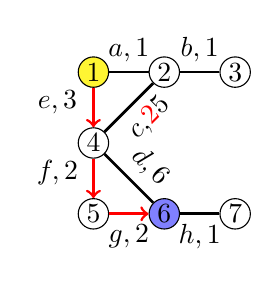
\begin{tikzpicture}
                \tikzset{Vertex/.style={%
                    shape=circle,%
                    draw=black,%
                    minimum size=10pt,%
                    radius=0.7cm,%
                    inner sep=1pt,%
                    node distance=0.9cm,%
                }}
            
                \node[Vertex, fill=yellow!80] (1) {$1$};
                \node[Vertex, right of=1] (2) {$2$};
                \node[Vertex, right of=2] (3) {$3$};
                \node[Vertex, below of=1] (4) {$4$};
                \node[Vertex, below of=4] (5) {$5$};
                \node[Vertex, right of=5, fill=blue!50] (6) {$6$};
                \node[Vertex, right of=6] (7) {$7$};
        
                \path (2) edge[-,line width=1pt] node[above]{\color{black}$a,1$} (1);
                \path (2) edge[-,line width=1pt] node[above]{\color{black}$b,1$} (3);
                \path (2) edge[-,line width=1pt] node[below,sloped,pos=0.4]{{\color{black} $c,$}{\color{red} \xcancel{2}}{\color{black}5}} (4);
                \path (4) edge[-,line width=1pt] node[above,sloped,pos=0.6]{\color{black}$d,6$} (6);
                \path (1) edge[->,line width=1pt, color=red] node[above,xshift=-13pt,yshift=-6pt]{\color{black}$e,3$} (4);
                \path (4) edge[->,line width=1pt, color=red] node[above,xshift=-13pt, yshift=-6pt]{\color{black}$f,2$} (5);
                \path (5) edge[->,line width=1pt, color=red] node[below]{\color{black}$g,2$} (6);
                \path (6) edge[-,line width=1pt] node[below]{\color{black}$h,1$} (7);
            \end{tikzpicture}
        \end{minipage}
    }%
    \only<5>{
        \begin{minipage}{0.65\textwidth}
            For every search node $n$, CPD allows us to track an incumbent solution which is the shortest such path we have found (\textit{upperbound}).
        \end{minipage}\hfill%
        \begin{minipage}{0.35\textwidth}
            \begin{center}
                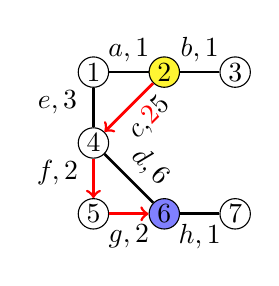
\begin{tikzpicture}
                    \tikzset{Vertex/.style={%
                        shape=circle,%
                        draw=black,%
                        minimum size=10pt,%
                        radius=0.7cm,%
                        inner sep=1pt,%
                        node distance=0.9cm,%
                    }}
                
                    \node[Vertex] (1) {$1$};
                    \node[Vertex, right of=1, fill=yellow!80] (2) {$2$};
                    \node[Vertex, right of=2] (3) {$3$};
                    \node[Vertex, below of=1] (4) {$4$};
                    \node[Vertex, below of=4] (5) {$5$};
                    \node[Vertex, right of=5, fill=blue!50] (6) {$6$};
                    \node[Vertex, right of=6] (7) {$7$};
            
                    \path (2) edge[-,line width=1pt] node[above]{\color{black}$a,1$} (1);
                    \path (2) edge[-,line width=1pt] node[above]{\color{black}$b,1$} (3);
                    \path (2) edge[->,line width=1pt, color=red] node[below,sloped,pos=0.4]{{\color{black} $c,$}{\color{red} \xcancel{2}}{\color{black}5}} (4);
                    \path (4) edge[-,line width=1pt] node[above,sloped,pos=0.6]{\color{black}$d,6$} (6);
                    \path (1) edge[-,line width=1pt] node[above,xshift=-13pt,yshift=-6pt]{\color{black}$e,3$} (4);
                    \path (4) edge[->,line width=1pt, color=red] node[above,xshift=-13pt, yshift=-6pt]{\color{black}$f,2$} (5);
                    \path (5) edge[->,line width=1pt, color=red] node[below]{\color{black}$g,2$} (6);
                    \path (6) edge[-,line width=1pt] node[below]{\color{black}$h,1$} (7);
                \end{tikzpicture}
            \end{center}
        \end{minipage}
    }
\end{frame}


\begin{frame}{Proposed technique: \CPDSearch{}}
    \textbf{\CPDSearch{}}. A* variant yielding bounded suboptimal path:
    \begin{itemize}
        \item mantain shortest incumbent path $I$ and its cost $u = g[I] + h'$ ($h'$ = \CPD{} path cost from $I$ to target over perturbated map);
        \item if $\epsilon f[n] \geq u$, output solution;
        \item when $\epsilon = 1$, \CPDSearch{} is optimal;
    \end{itemize}

    heuristic used: cost of \CPD{} path;
    
\end{frame}

\begin{frame}{\CPDSearch{} as anytime algorithm}
    \begin{itemize}
        \item each node in openlist represents an actual solution as well (if new weights $\not = \infty$); 
        \item \CPD{} provides both lowerbound and upperbound of solution;
        \item Anytime variant obtained by yielding every incumbents $I$ \CPDSearch{} finds;
        \item Often the first incumbent is calculated from the start node $\Rightarrow$ fast first incumbent;
    \end{itemize}
\end{frame}